\documentclass[tikz,border=5pt]{standalone}
\usepackage{xcolor}
\usetikzlibrary{arrows.meta,calc}

\begin{document}
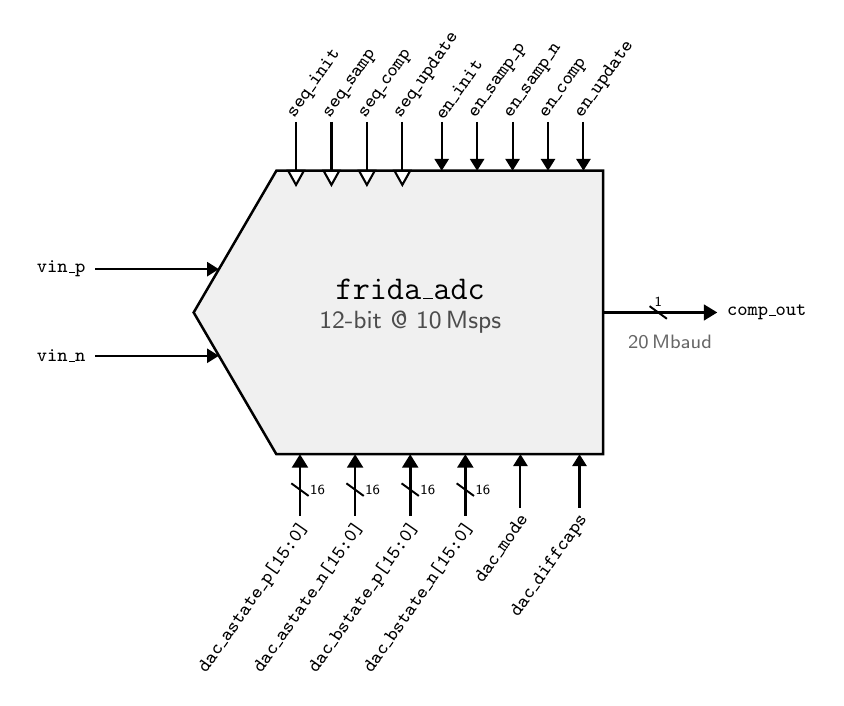
\begin{tikzpicture}[
  font=\sffamily\small,
  signal/.style={font=\ttfamily\scriptsize},
  pin/.style={line width=0.75pt},
  input/.style={-{Triangle[length=1.5mm,width=1.8mm]}, line width=0.75pt},
  output/.style={-{Triangle[length=1.7mm,width=2.0mm]}, line width=0.75pt},
  bus/.style={-{Triangle[length=1.7mm,width=2.0mm]}, line width=1.0pt},
]
  % ADC body: conventional converter symbol with a pointed analog-input side.
  \coordinate (tip) at (-2.9,0);
  \coordinate (nw) at (-1.85,1.8);
  \coordinate (ne) at ( 2.3,1.8);
  \coordinate (se) at ( 2.3,-1.8);
  \coordinate (sw) at (-1.85,-1.8);
  \draw[fill=black!6, line width=0.9pt]
    (tip) -- (nw) -- (ne) -- (se) -- (sw) -- cycle;

  \node[font=\ttfamily\bfseries\large] at (-0.15,0.30) {frida\_adc};
  \node[font=\sffamily\small, text=black!70] at (-0.15,-0.12)
    {12-bit @ 10\,Msps};

  % Differential analog input.
  \draw[input]
    (-4.15,0.55) -- (-2.58,0.55);
  \draw[input]
    (-4.15,-0.55) -- (-2.58,-0.55);
  \node[signal, left] at (-4.15,0.55) {vin\_p};
  \node[signal, left] at (-4.15,-0.55) {vin\_n};

  % Single-bit comparator result.
  \draw[output]
    (2.3,0) -- (3.75,0);
  \node[signal, right] at (3.75,0) {comp\_out};
  \draw[line width=0.7pt] (2.89,0.08) -- (3.11,-0.08);
  \node[font=\sffamily\tiny, anchor=south, inner sep=0.5pt]
    at (3.0,0.045) {1};
  \node[font=\sffamily\scriptsize, text=black!60, below]
    at (3.15,-0.16) {20\,Mbaud};

  % Four sequencer phases, marked with clock-edge triangles.
  \foreach \x/\name in {
    -1.60/seq\_init,
    -1.15/seq\_samp,
    -0.70/seq\_comp,
    -0.25/seq\_update
  } {
    \draw[pin] (\x,2.42) -- (\x,1.8);
    \draw[pin, fill=white]
      ({\x-0.10},1.8) -- (\x,1.62) -- ({\x+0.10},1.8) -- cycle;
    \node[signal, rotate=55, anchor=south west, inner sep=0.5pt]
      at ({\x+0.03},2.40) {\name};
  }

  % Five local enables.
  \foreach \x/\name in {
     0.25/en\_init,
     0.70/en\_samp\_p,
     1.15/en\_samp\_n,
     1.60/en\_comp,
     2.05/en\_update
  } {
    \draw[input]
      (\x,2.42) -- (\x,1.8);
    \node[signal, rotate=55, anchor=south west, inner sep=0.5pt]
      at ({\x+0.03},2.40) {\name};
  }

  % Configuration inputs.
  \foreach \x/\name in {
    -1.55/dac\_astate\_p[15:0],
    -0.85/dac\_astate\_n[15:0],
    -0.15/dac\_bstate\_p[15:0],
     0.55/dac\_bstate\_n[15:0]
  } {
    \draw[bus] (\x,-2.58) -- (\x,-1.8);
    \draw[line width=0.7pt]
      ({\x-0.11},-2.17) -- ({\x+0.11},-2.33);
    \node[font=\sffamily\tiny, right, inner sep=0.5pt]
      at ({\x+0.105},-2.25) {16};
    \node[signal, rotate=55, anchor=north east, inner sep=0.5pt]
      at ({\x-0.03},-2.59) {\name};
  }

  \draw[input] (1.25,-2.48) -- (1.25,-1.8);
  \node[signal, rotate=55, anchor=north east, inner sep=0.5pt]
    at (1.22,-2.50) {dac\_mode};

  \draw[input] (2.0,-2.48) -- (2.0,-1.8);
  \node[signal, rotate=55, anchor=north east, inner sep=0.5pt]
    at (1.97,-2.50) {dac\_diffcaps};
\end{tikzpicture}
\end{document}
